
\todo[inline]{Here, it seemed more important to show multiple error metrics
than with the first experiment. That may or may not be true. Was planning on
including some error histograms of certain cases to motive it here. }

\subsubsection{Burnup Regression}

\begin{figure}[!htb]
  \centering
  \begin{subfigure}[b]{\textwidth}
    \centering
    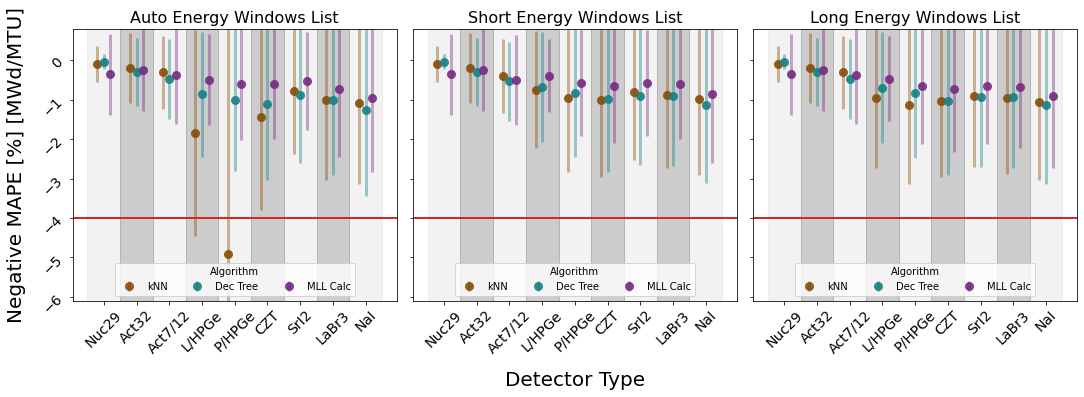
\includegraphics[width=\textwidth]{./chapters/exp2/detector_preds_wrt_enlist_MAPE_burn.png}
    \caption{Prediction performance measured by \gls{MAPE}.}
    \label{fig:burnA}
  \end{subfigure}
  \vskip\baselineskip
  \begin{subfigure}[b]{\textwidth}
    \centering
    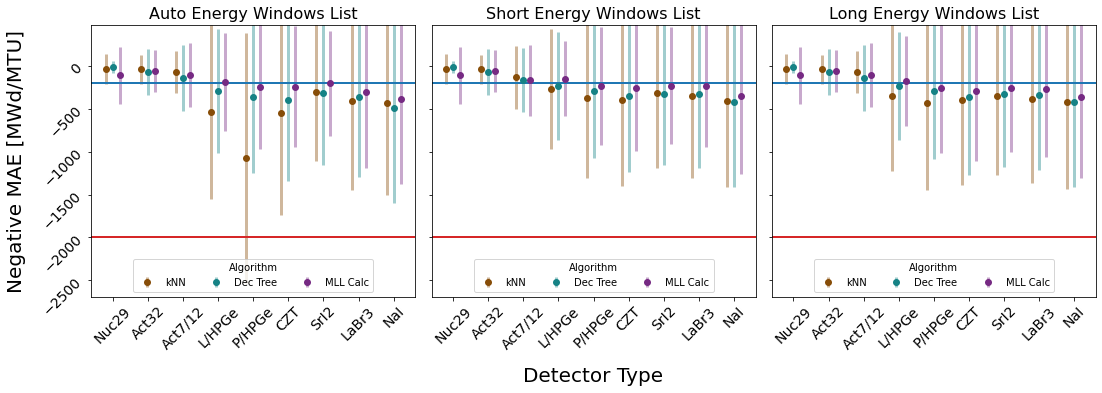
\includegraphics[width=\textwidth]{./chapters/exp2/detector_preds_wrt_enlist_MAE_burn.png}
    \caption{Prediction performance measured by \gls{MAE}.} 
    \label{fig:burnB}
  \end{subfigure}
  \vskip\baselineskip
  \begin{subfigure}[b]{\textwidth}
    \centering
    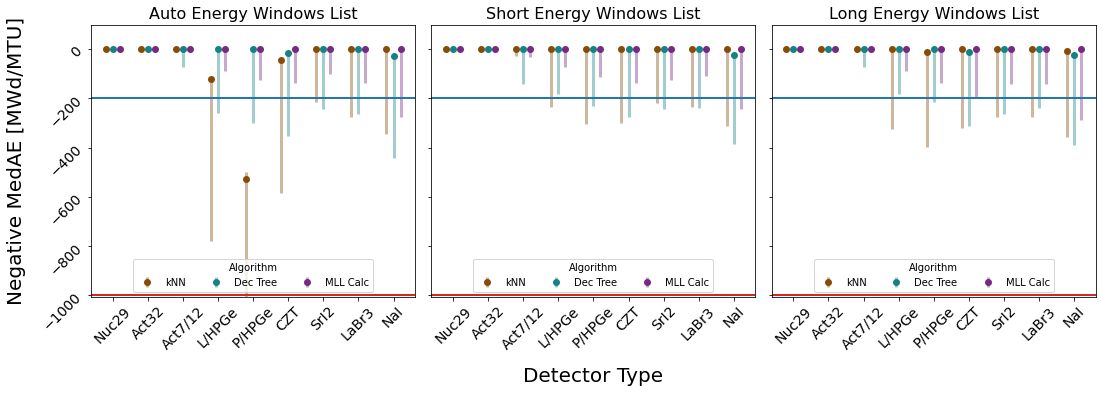
\includegraphics[width=\textwidth]{./chapters/exp2/detector_preds_wrt_enlist_MedAE_burn.png}
    \caption{Prediction performance measured by \gls{MedAE}.}
    \label{fig:burnC}
  \end{subfigure}
  \caption{Prediction performance of burnup with respect to decreasing detector 
           energy resolution for three types of processed gamma spectra.}
  \label{fig:burn}
\end{figure}

\subsubsection{U235 Enrichment Regression}

\begin{figure}[!htb]
  \centering
  \begin{subfigure}[b]{\textwidth}
    \centering
    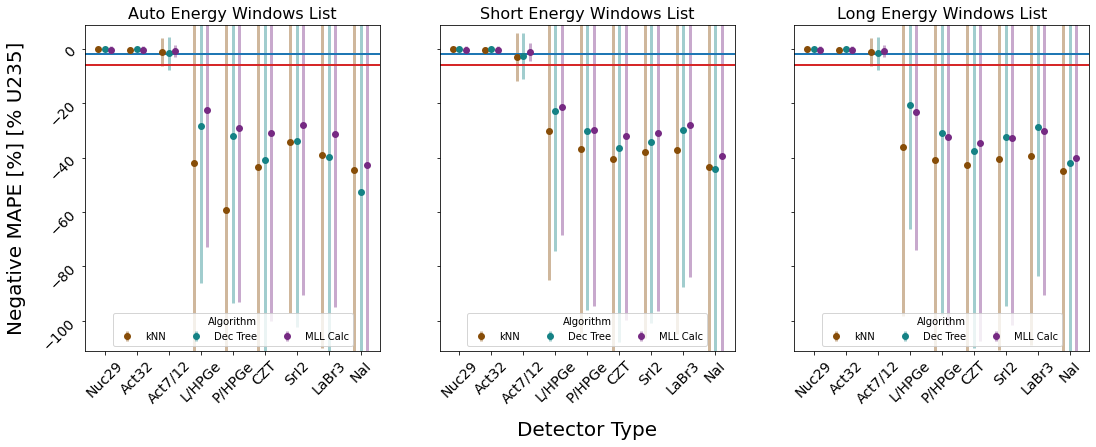
\includegraphics[width=\textwidth]{./chapters/exp2/detector_preds_wrt_enlist_MAPE_enri.png}
    \caption{Prediction performance measured by \gls{MAPE}.}
    \label{fig:enriA}
  \end{subfigure}
  \vskip\baselineskip
  \begin{subfigure}[b]{\textwidth}
    \centering
    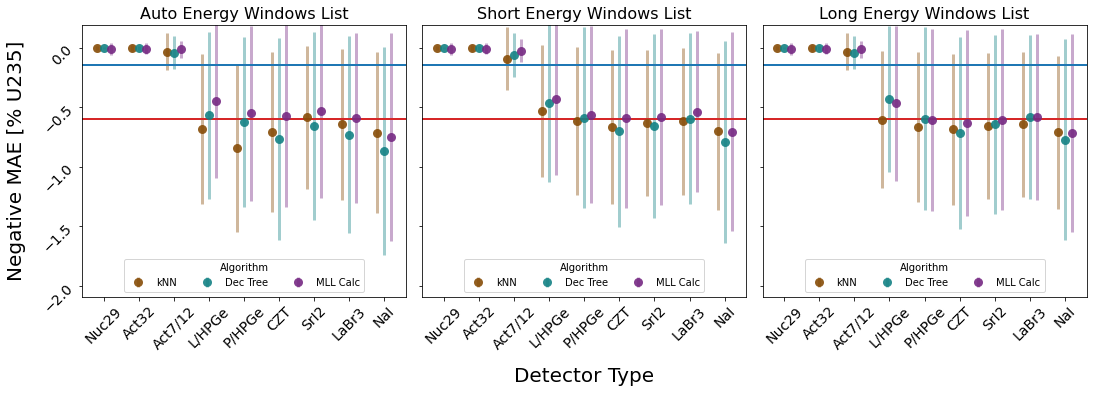
\includegraphics[width=\textwidth]{./chapters/exp2/detector_preds_wrt_enlist_MAE_enri.png}
    \caption{Prediction performance measured by \gls{MAE}.} 
    \label{fig:enriB}
  \end{subfigure}
  \vskip\baselineskip
  \begin{subfigure}[b]{\textwidth}
    \centering
    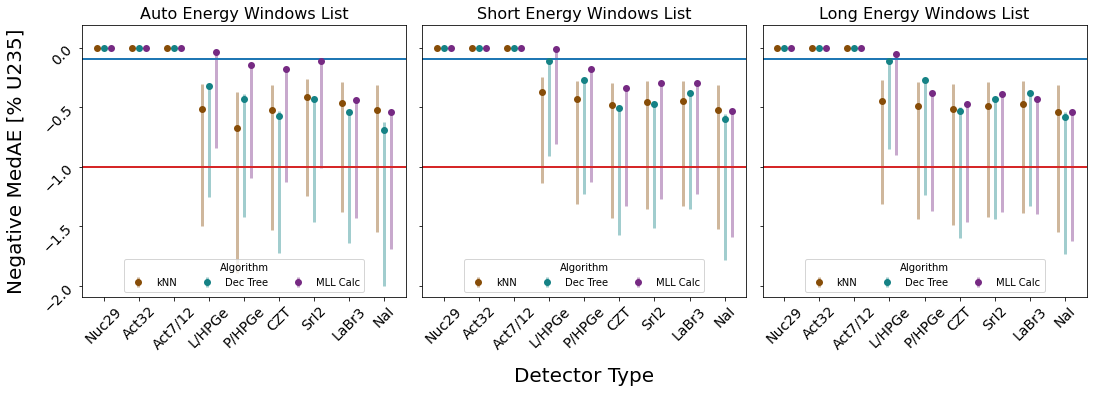
\includegraphics[width=\textwidth]{./chapters/exp2/detector_preds_wrt_enlist_MedAE_enri.png}
    \caption{Prediction performance measured by \gls{MedAE}.}
    \label{fig:enriC}
  \end{subfigure}
  \caption{Prediction performance of enrichment with respect to decreasing 
           detector energy resolution for three types of processed gamma 
           spectra.}
  \label{fig:enri}
\end{figure}

\subsubsection{Time Since Irradiation Regression}

\begin{figure}[!htb]
  \centering
  \begin{subfigure}[b]{\textwidth}
    \centering
    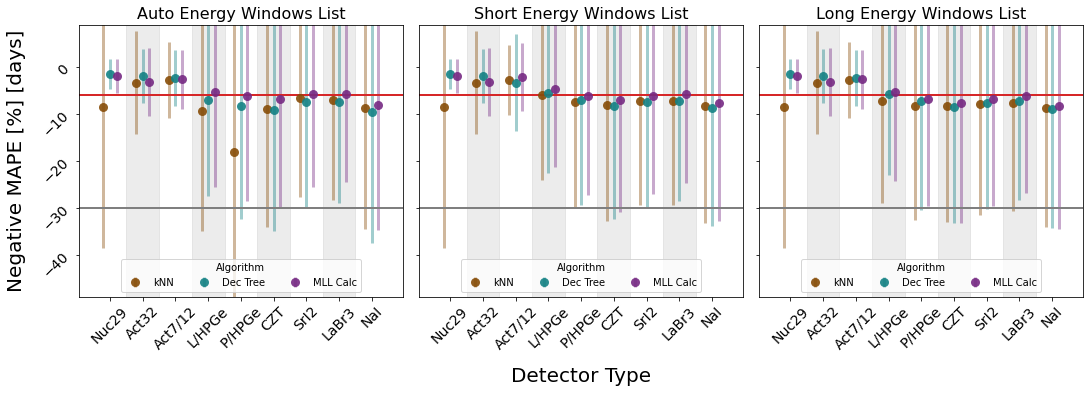
\includegraphics[width=\textwidth]{./chapters/exp2/detector_preds_wrt_enlist_MAPE_cool.png}
    \caption{Prediction performance measured by \gls{MAPE}.}
    \label{fig:coolA}
  \end{subfigure}
  \vskip\baselineskip
  \begin{subfigure}[b]{\textwidth}
    \centering
    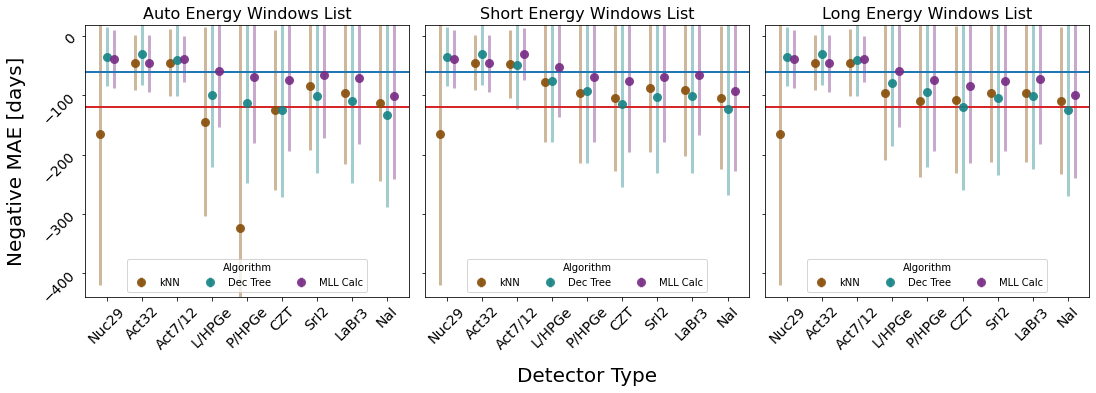
\includegraphics[width=\textwidth]{./chapters/exp2/detector_preds_wrt_enlist_MAE_cool.png}
    \caption{Prediction performance measured by \gls{MAE}.} 
    \label{fig:coolB}
  \end{subfigure}
  \vskip\baselineskip
  \begin{subfigure}[b]{\textwidth}
    \centering
    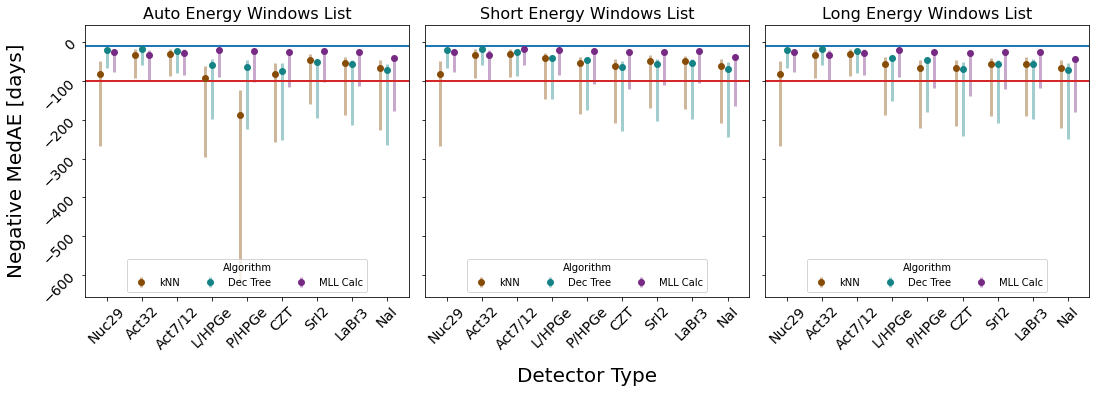
\includegraphics[width=\textwidth]{./chapters/exp2/detector_preds_wrt_enlist_MedAE_cool.png}
    \caption{Prediction performance measured by \gls{MedAE}.}
    \label{fig:coolC}
  \end{subfigure}
  \caption{Prediction performance of time since irradiation with respect to 
           decreasing detector energy resolution for three types of processed 
           gamma spectra.}
  \label{fig:cool}
\end{figure}

